\begin{figure}[t]
\centering
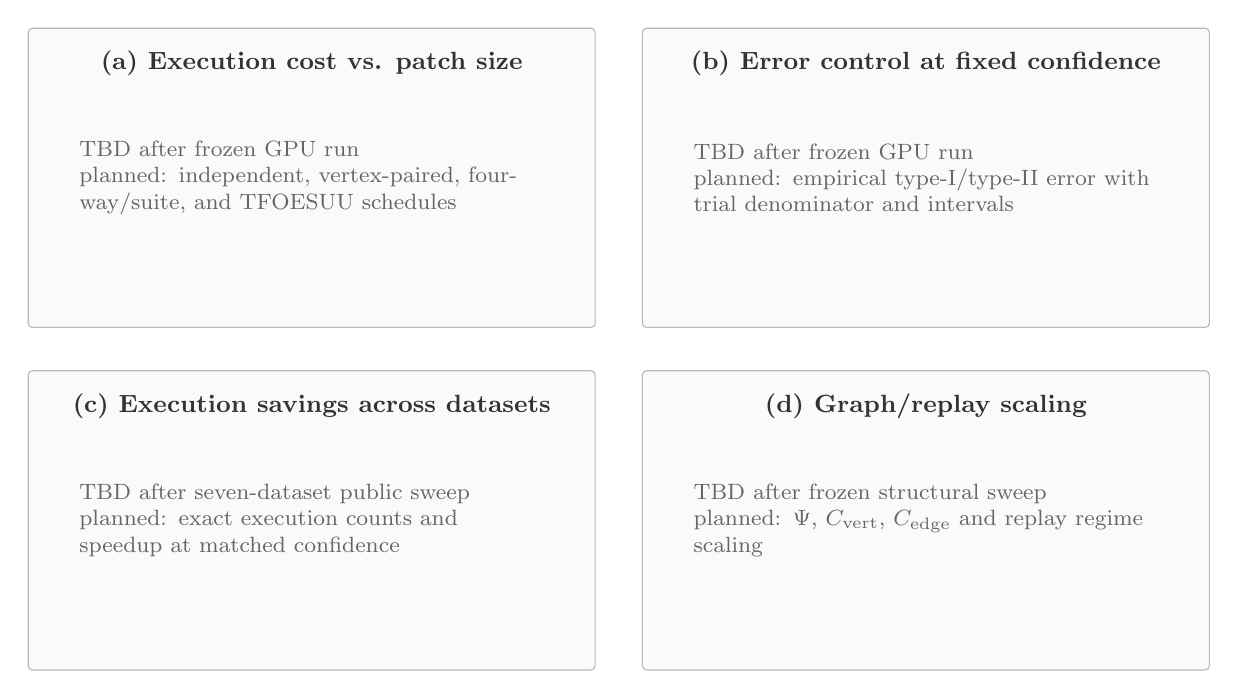
\begin{tikzpicture}[
  panel/.style={draw=black!28, rounded corners=1.5pt, fill=black!2,
               minimum width=7.2cm, minimum height=3.8cm, align=center},
  ttl/.style={font=\small\bfseries, text=black!80},
  sub/.style={font=\footnotesize, text=black!60}
]
\node[panel] (a) at (0,0) {};
\node[ttl] at ([yshift=1.45cm]a.center) {(a) Execution cost vs. patch size};
\node[sub, text width=5.9cm] at (a.center) {TBD after frozen GPU run\\
planned: independent, vertex-paired, four-way/suite, and TFOESUU schedules};

\node[panel] (b) at (7.8,0) {};
\node[ttl] at ([yshift=1.45cm]b.center) {(b) Error control at fixed confidence};
\node[sub, text width=5.9cm] at (b.center) {TBD after frozen GPU run\\
planned: empirical type-I/type-II error with trial denominator and intervals};

\node[panel] (c) at (0,-4.35) {};
\node[ttl] at ([yshift=1.45cm]c.center) {(c) Execution savings across datasets};
\node[sub, text width=5.9cm] at (c.center) {TBD after seven-dataset public sweep\\
planned: exact execution counts and speedup at matched confidence};

\node[panel] (d) at (7.8,-4.35) {};
\node[ttl] at ([yshift=1.45cm]d.center) {(d) Graph/replay scaling};
\node[sub, text width=5.9cm] at (d.center) {TBD after frozen structural sweep\\
planned: $\Psi$, $C_{\rm vert}$, $C_{\rm edge}$ and replay regime scaling};
\end{tikzpicture}
\caption{Pre-registered result-figure layout. The four panels are placeholders,
not evidence. They will be generated automatically from frozen result JSONL
after the local publication run; no hand-entered numerical values are permitted.}
\label{fig:public-results-tbd}
\end{figure}